\documentclass[a4paper,11pt]{article}
\input{/home/tof/Documents/Cozy/latex-include/preambule_lua.tex}
\newcommand{\showprof}{show them}  % comment this line if you don't want to see todo environment
\fancyhead[L]{Portes logiques}
\newdate{madate}{10}{09}{2020}
\fancyhead[R]{Première - NSI} %\today
\fancyfoot[L]{~\\Christophe Viroulaud}
\fancyfoot[C]{\textbf{Page \thepage}}
\fancyfoot[R]{\includegraphics[width=2cm,align=t]{/home/tof/Documents/Cozy/latex-include/cc.png}}

\begin{document}
\begin{Form}
\paragraph{Objectif:}Découvrir les fonctions booléennes.
\section{Problématique}
En 1965 puis 1975, les lois de Moore prédisent que le nombre de transistors des microprocesseurs double tous les deux ans.
\begin{figure}[!h]
\centering
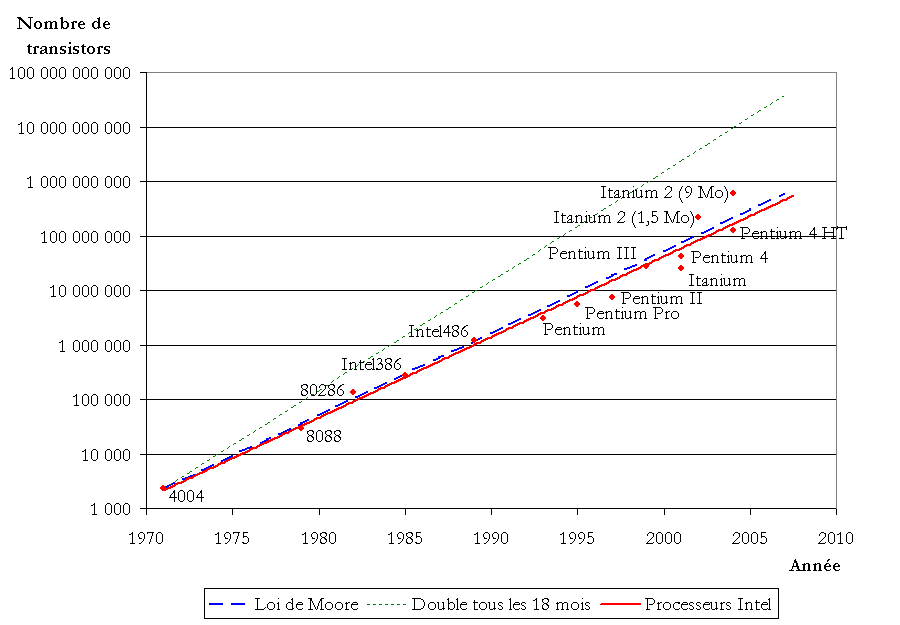
\includegraphics[width=10cm]{ressources/loi-moore.png}
\captionof{figure}{Loi de Moore}
\label{moore}
\end{figure}
\\Mais il ne suffit pas de graver de plus en plus finement pour construire un microprocesseur.
\begin{commentprof}
On détermine la qualité de la gravure selon le plus petit motif qu'il est possible de graver, en l'occurrence la largeur de la grille du transistor MOS: 2004 = 130nm, 2018 = 10nm.
\end{commentprof}
\begin{center}
\shadowbox{\parbox{14cm}{\centering Comment utiliser les propriétés d'un transistor pour effectuer des calculs?}}
\end{center}
\begin{commentprof}
\section*{Retour historique}
Babbage reprend notamment l'idée des cartes perforées pour programmer sa machine.\\diode à vide composée de:
\begin{itemize}
\item cathode: émet électron
\item anode: capte électron
\item fil tungstène: pour chauffer
\end{itemize}
Le courant maximum pouvant traverser la diode dépend de la nature de la cathode et de sa température.\\1906: le courant circulant du filament vers la plaque (anode) dépend de la tension appliquée sur la grille. Le principe du transistor est né.\\atanasoff: testé avec succès en 42. suivent colossus (cryptanalyse),ENIAC, UNIVAC 1)\\transistor: à partir des années 50: moins cher et plus fiable.\\TRADIC: 700 transistors et 10 000 diodes.\\4004: 2300 transistors 
\end{commentprof}
\section{Portes logiques}
\begin{commentprof}
Il y a plusieurs façons de créer les différentes portes. Selon simplicité, économie de transistors...
\end{commentprof}
\subsection{Principe du transistor}
Un transistor se comporte comme un interrupteur qui laisse ou non passer le courant sur le principe du \emph{tout ou rien}.
\begin{figure}[!h]
\centering
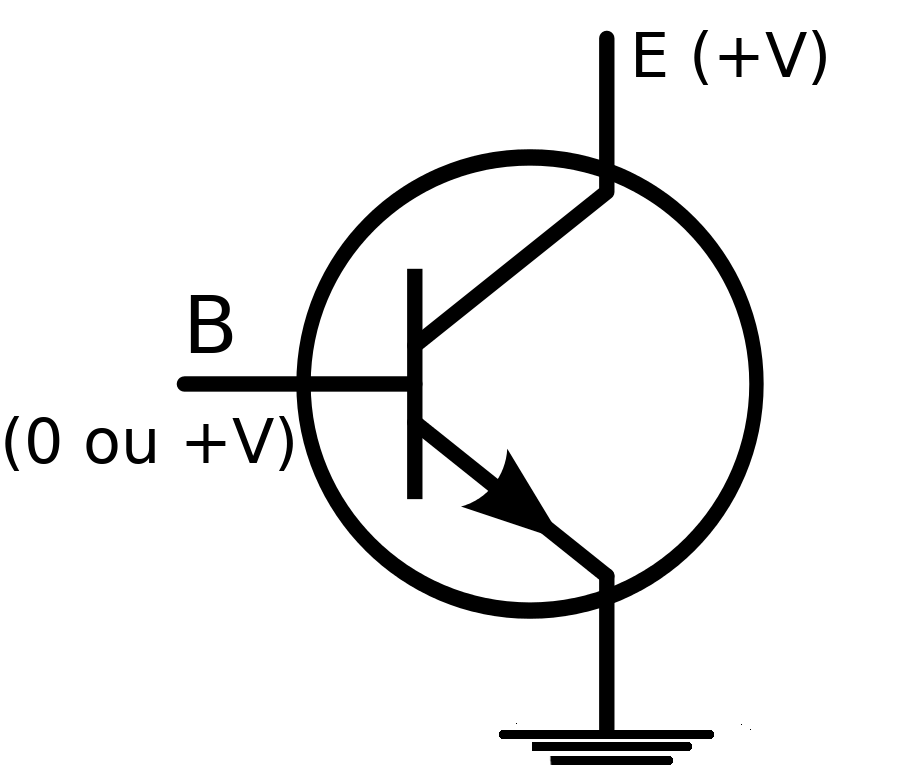
\includegraphics[width=5cm]{ressources/transistor-schema.png}
\captionof{figure}{Le transistor}
\label{transistor}
\end{figure}
\\La broche B joue le rôle de la commande d'interrupteur:
\begin{itemize}
\item Lorsqu'elle est sous tension, elle laisse passer le courant entre la broche E est la masse: la broche E passe sous tension basse.
\item Lorsqu'elle est sous tension basse, la broche E reste sous tension haute.
\end{itemize}
\begin{commentprof}
logique binaire: déjà utilisée avec carte perforée, tube à vide. ici le passage du courant électrique ou non == trou dans carte ou pas; + logique booléenne
\end{commentprof}
\subsection{Première porte logique: NON}
Une porte logique est une fonction qui accepte un ou plusieurs bits en entrée et qui produit un bit en sortie.\\Le transistor (figure \ref{transistor}) permet de réaliser une opération élémentaire:
\begin{center}
\begin{tabular}{*{2}{>{\centering\arraybackslash}m{.4\textwidth}}}
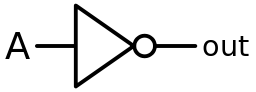
\includegraphics[width=5cm]{ressources/not-us.png}
  & 
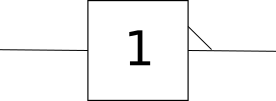
\includegraphics[width=5cm]{ressources/not-eu.png}  
   \\
Symbole américain & Symbole européen
\end{tabular}
\end{center}
La table logique (table de vérité) représente le calcul réalisé par une porte logique:
\begin{table}[!h]
\begin{center}
\begin{tabular}{|c|c|}
\hline 
Entrée & Sortie \\ 
\hline 
1 & 0 \\ 
\hline 
0 & 1 \\ 
\hline 
\end{tabular}
\caption{\label{not}Fonction NON}
\end{center}
\end{table} 
\end{Form}
\end{document}